%\begin{savequote}[10cm]
%{\it ``The Three Laws of Robotics: \\
%1: A robot may not injure a human being or, through inaction, allow a human being to come to harm; \\
%2: A robot must obey the orders given it by human beings except where such orders would conflict with the First Law;\\
%3: A robot must protect its own existence as long as such protection does not conflict with the First or Second Law.''}
%\qauthor{Isaac Asimov}
%\end{savequote}

\chapter{Introduction} 
\label{Chap:Introduction}

This thesis was made with the spirit of contributing to the autonomy of humanoid robots; more precisely in the development of behaviors based on computer vision. Even with the tremendous expansion of humanoid robotics in the last years, the link between perception and motion generation is still not well developed. Hundreds of works cover both fields separately. In the perception side, computer vision is up to this day the main technique in humanoid robotics. 

On the robotic side, there is an increasing interest in the development of humanoid robotics. Governments and companies such as Honda, Boston Dynamics and Aldebaran Robotics have spent a lot of money in these fields. As a result, amazing demonstrations in humanoid motion generation have been done recently. However, the interaction with the environment is limited in most of the systems.

%% main text
The design of humanoid robots has been done thinking mainly in human-friendly environments, i.e. unstructured and dynamic environments, where objects move outside the robots control. Therefore, when specific tasks have to be completed, these robots have to be able to perceive and react to environmental changes. Visual sensors can help them to reach this objective, by allowing to build local representations of the robot surroundings, and to adapt their behavior in consequence. Most of the existing humanoid platforms are equipped with video cameras, providing the robots with rich information (geometry, texture, color\dots) without adding so much weight and size, at a rather low cost. Moreover, the use of embedded cameras is attractive because it avoids equipping the environment with additional external sensors. Such an embedding increases greatly the level of autonomy of the robotic platform. However, to interpret the data generated from the camera of a humanoid robot is still problematic, with a huge amount of undergoing work in the computer vision community, as, in general, the image quality in humanoid robots is quite poor: blurring effects or vibrations due to the walk may make visual tasks such as  localization and tracking really challenging. 

Early works on humanoid locomotion have assumed that the robot path is defined before computing the actual joint control to realize it. This clearly puts limits on the capacities of reaction when changes occur in the environment. These works generally follow a perception-decision-action scheme, in the sense that a sensor first acquires data on the world and/or the robot state, then, suitable footsteps over a time horizon are decided, and finally the trajectories of the Center of Mass (CoM) and the Center of Pressure (CoP) are computed while respecting the stability constraints and avoiding collision with the environment. Finally, the control of the legs and other joints is computed by inverse kinematics, given the previously computed CoM trajectory, and the sequence of footsteps to follow. This perception-decision-action loop has proven to be fast enough  to realize impressive demonstrations for stair-climbing and obstacle avoidance. Our focus in this thesis will be set only on one of the sub-problems necessary to implement this approach: the generation of footsteps and trajectories of the CoM and CoP. We stress that we will not address here the whole body control.


A general diagram of the workflow in humanoid robots is depicted in Fig.~\ref{Fig:GeneralDiagram}. In general we use computer vision to extract information from the environment (mapping, localization, modeling). With this model, we can plan the motion using rules given by a cognitive process. With this plan, the robot performs the dynamic walking which leads to the whole body motion. Computer vision requires high computational load to extract high level information from the scene; motion generation on the other side, requires fast control loops to be dynamically stable. 

\begin{figure}[h!]
\centering
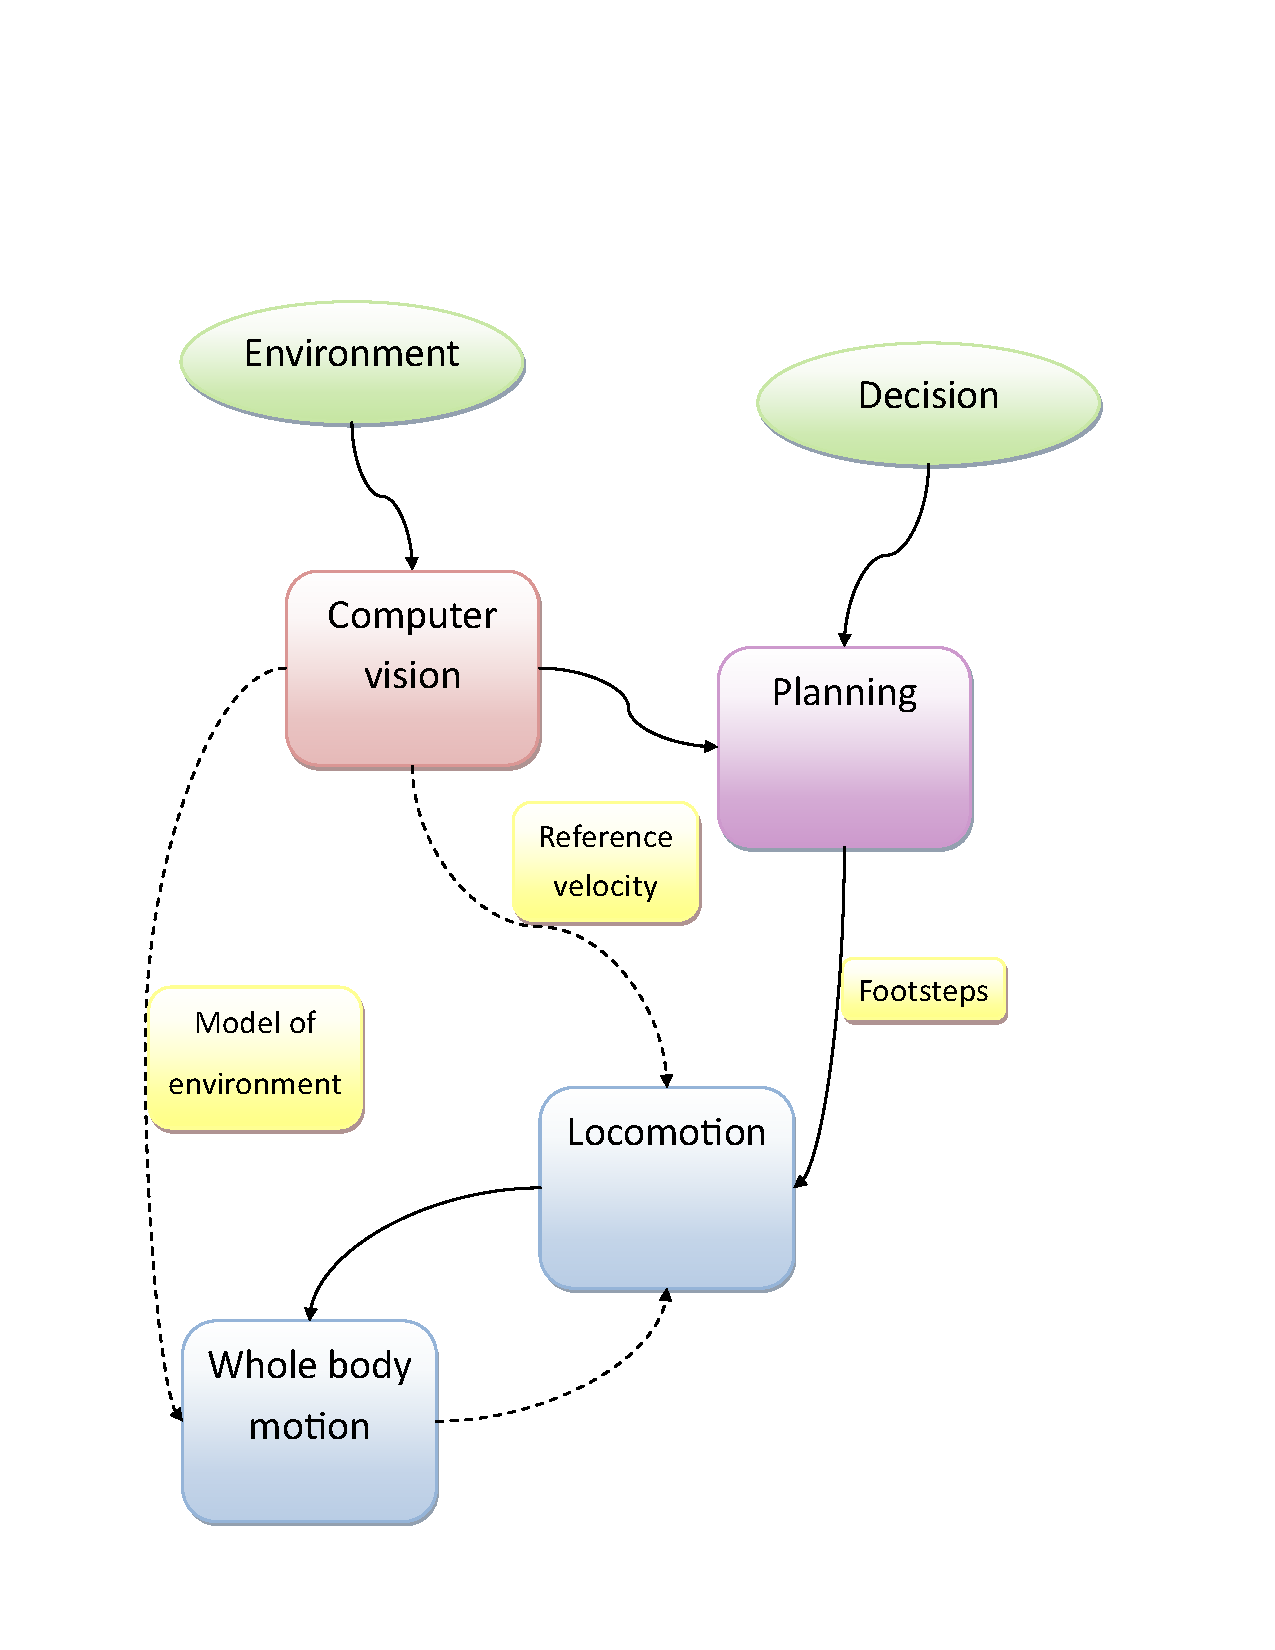
\includegraphics[scale=0.5]{Chap1-Introduction/general-diagram.pdf}
\caption[]{ \label{Fig:GeneralDiagram} Workflow of a humanoid robot executing motion tasks using perception.}
\end{figure}

In this thesis we address the problem of the link between vision and motion generation, as illustrated in Fig~\ref{Fig:PhotosVS}. Building upon the work of several authors through the years, our main contributions are,

\begin{itemize}
\item The full integration of a visual servoing scheme within the walking motion generation using Linear Model Predictive Control (MPC);
\item The integration of traditional motion planning approaches and on-line locomotion generation algorithms;
\item The visual reconstruction of 3D models of the scene in front of the robot to be used by an inverse-dynamics based approach to walk on rough terrain;
\item And finally, the validation in simulation of the proposals.
\end{itemize}

\begin{figure}[h!]
\centering
\subfigure[]{
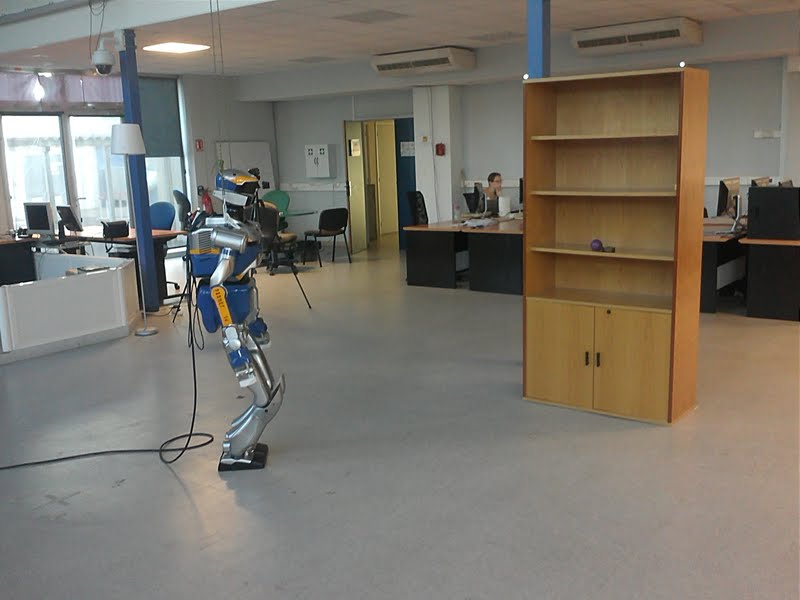
\includegraphics[scale=0.3]{Chap1-Introduction/hrp_2_setup.jpeg}}
\subfigure[]{
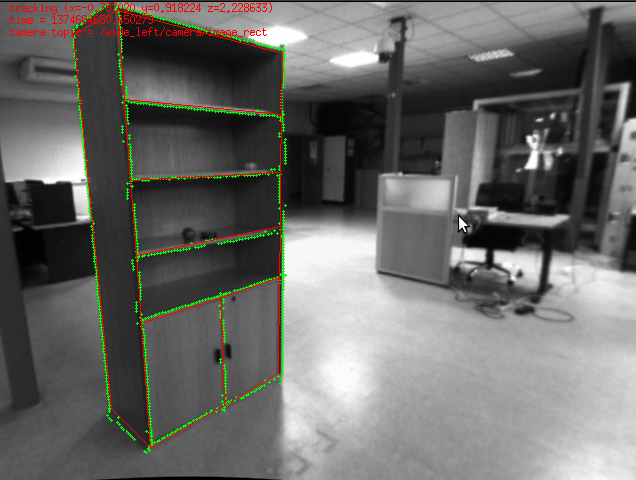
\includegraphics[scale=0.375]{Chap1-Introduction/visp_tracker_hrp2_big_shelf.png}}
\caption[]{ \label{Fig:PhotosVS} Typical application of computer vision and control, visual servoing.}
\end{figure}


The rest of this manuscript is organized as follows. In chapter \ref{Chap:Related-Work}, we state the problem and briefly recall the work that has been done on it. In chapter \ref{Chap:Locomotion-Control}, we introduce the techniques that most of the current walking motion generation schemes for humanoid robots are based on. The one proposed in Kajita et al. in 2003 \citep{Kajita2003} that focuses in the trajectory of the center of mass to generate balanced and stable motions and the one proposed by Herdt et al. in 2010 \citep{HerdtAR2010} in which a reference velocity is tracked. In chapter \ref{Chap:Visual-Servoing} we present an approach to introduce visual information in the walking pattern generator for humanoid robots. We make use of visual servoing with Model Predictive Control (MPC), which is combined with the walking motion generator. Since visual servoing with MPC is in general a nonlinear optimization problem, we propose a linearization scheme in order to keep it as a Quadratic Program (QP) and introduce it within the pattern generator. In chapter \ref{Chap:Visual-Planning}, we propose a method for reactive walking allowing visual servoing and adaptation of footsteps trajectories in real-time. This is done by building upon recent advances in the fields of optimal control for a walking pattern generator~\citep{HerdtAR2010} and planning for a nonholomic robot with field-of-view constraints ~\citep{Salaris:2010}. In chapter \ref{Chap:3DReconstruction}, we present a 3D reconstruction system of the ground in front of the robot. This model allows to know the ground structure where the swinging foot is going to step on to an inverse dynamics control scheme. Finally, in chapter \ref{Chap:Conclusions}, we present the final discussion and future work.


